\subsection{XOR}
    The XOR gate, short for Exclusive OR, represents the expression $(A\cdot {\overline {B}})+({\overline {A}}\cdot B)$.
    It can be constructed using AND, OR and NOT gates, however, this approach would require five gates of three different kinds. 
    As an alternative, the XOR gate can be made of just universal gates: from four NAND gates, as shown in Figure \ref{fig:XOR_gate1}, or from five NOR gates, as shown in Figure \ref{fig:XOR_gate2}. \\\\	
    \begin{figure}[H]   
        \begin{minipage}{0.5\textwidth}
            \centering
            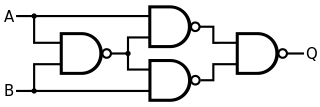
\includegraphics[width=0.8\textwidth]{figures/circuits/XOR_from_NAND.png}
            \captionof{figure}{XOR gate from NAND gates.} 
            \label{fig:XOR_gate1} 
        \end{minipage}
        \begin{minipage}{0.5\textwidth}
            \centering
            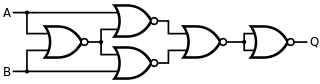
\includegraphics[width=1\textwidth]{figures/circuits/XOR_from_NOR.png}
            \captionof{figure}{XOR gate from NOR gates.} 
            \label{fig:XOR_gate2} 
        \end{minipage}
	\end{figure}
    
    \noindent
    An analytical representation of XOR gate could be $f(A,B)=A+B-2AB$. 
    The XOR gate gives a high output if one, and only one, of the inputs to the gate is high. 
    This behavior is consistent with the XOR gate's truth table shown in Table \ref{tab:XOR_table}. \\

    \begin{table}[ht]
        \centering
        \begin{tabular}{|c|c|c|}
            \hline
            Input A & Input B & Output \\
            \hline
            0 & 0 & 0 \\
            0 & 1 & 1 \\
            1 & 0 & 1 \\
            1 & 1 & 0 \\
            \hline
        \end{tabular}
        \caption{XOR truth table.}
        \label{tab:XOR_table}
    \end{table}   
    
    \begin{figure}[H]
	    \centering
	    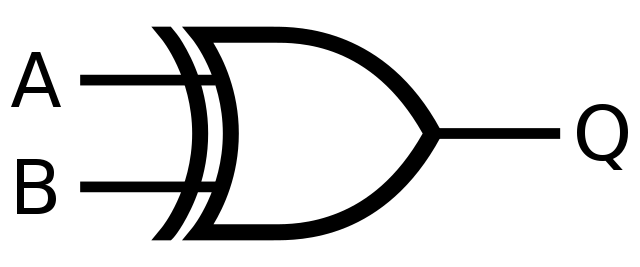
\includegraphics[width=0.3\textwidth]{figures/symbols/XOR.png}
	    \caption{XOR symbol.}
	    \label{fig:XOR_sym} 
	\end{figure}

    \noindent
    In the laboratory, it was used a different approach to build the XOR gate, using only four transistors, as shown in Figure \ref{fig:XOR_gate}.
    \begin{figure}[H]
        \centering
        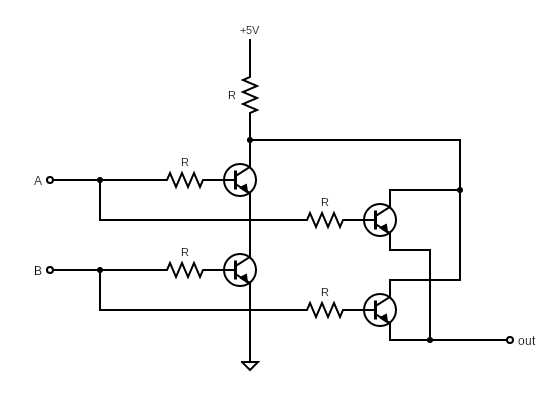
\includegraphics[width=0.5\textwidth]{figures/circuits/XOR.png}
        \caption{XOR gate.}
        \label{fig:XOR_gate}
    \end{figure}

    \noindent
    The following photographs show the XOR gate built in the laboratory and its behavior.
    \begin{figure}[H]
        \centering

        \begin{subfigure}{0.45\textwidth}
            \centering
            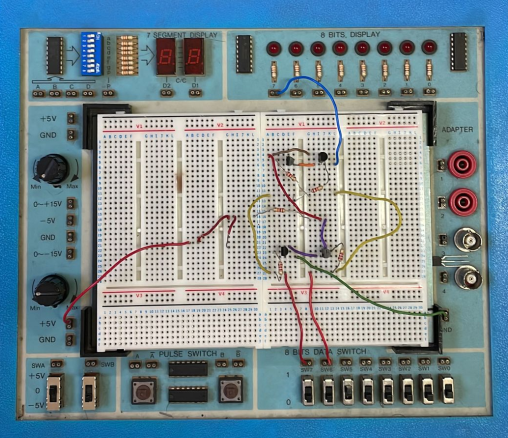
\includegraphics[width=\linewidth]{figures/photos/XOR/00.png}
            \caption{A = 0, B = 0}
        \end{subfigure}
        \hfill
        \begin{subfigure}{0.45\textwidth}
            \centering
            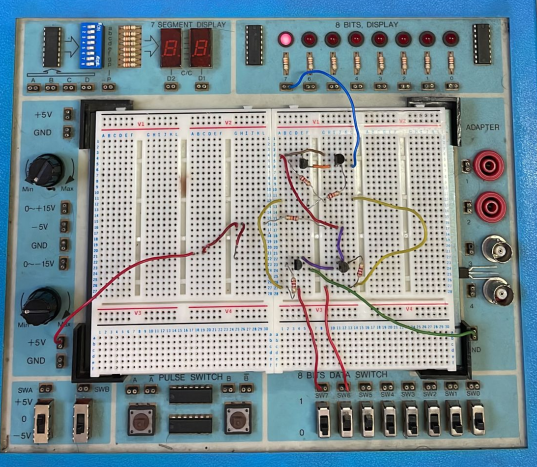
\includegraphics[width=\linewidth]{figures/photos/XOR/01.png}
            \caption{A = 0, B = 1}
        \end{subfigure}

        \vspace{1cm} % Adjust vertical space between rows

        \begin{subfigure}{0.45\textwidth}
            \centering
            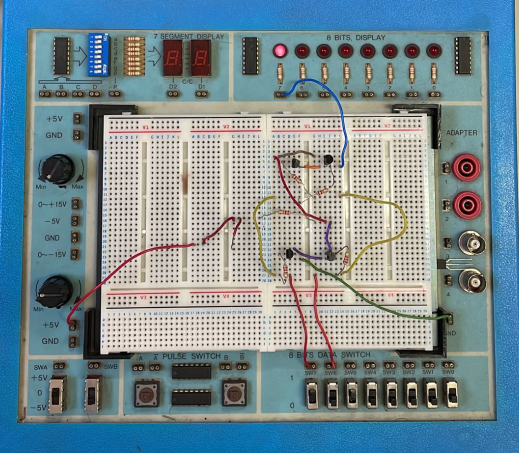
\includegraphics[width=\linewidth]{figures/photos/XOR/10.png}
            \caption{A = 1, B = 0}
        \end{subfigure}
        \hfill
        \begin{subfigure}{0.45\textwidth}
            \centering
            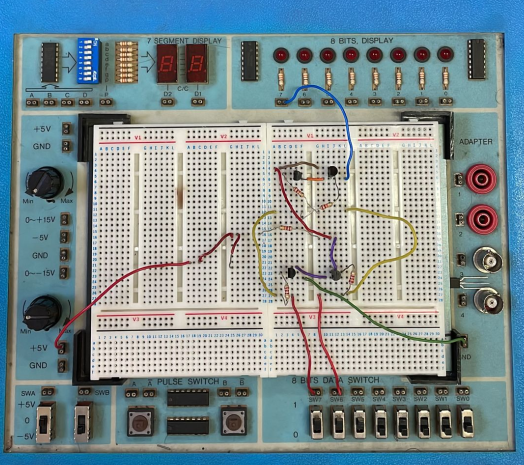
\includegraphics[width=\linewidth]{figures/photos/XOR/11.png}
            \caption{A = 1, B = 1}
        \end{subfigure}

        \caption{Four BJTs XOR gate constructed in the laboratory.}
        \label{fig:XOR_photos}
    \end{figure}
